\chapter{Analisis}
\label{chap:analisis}

Pada bab ini akan dibahas mengenai analisis perangkat lunak,

\section{Analisis Data}

Pada sub bab ini, akan dilakukan analisa tentang Twitter API, OAuth, KIRI API, dan Twitter4j. Setelah membaca dan menganalisis maka peneliti akan menentukan hal-hal  yang akan digunakan dalam membangun Twitter Bot untuk mencari jalur transportasi publik.

\subsection{Analisis Twitter API}
Setelah melakukan analisis, perangkat lunak yang akan dibangun akan menggunakan \textit{Streaming} API, karena:
\begin{itemize}
	\item Streaming API adalah \textit{real-time} API, sedangkan Search API hanya dapat menangkap tweet setiap beberapa waktu sekali.
	\item Menggunakan \textit{User Stream} dalam \textit{endpoint streaming}. User Stream mengandung hampir semua data yang berhubungan dengan satu user tertentu. Dalam pembuatan Twitter Bot untuk mencari jalur transportasi publik pengguna hanya dapat melakukan \textit{mention tweet} kepada user @kiriupdate untuk dapat memperoleh balasan tweet yang berisikan hasil pencarian jalur transportasi publik.
\end{itemize}

\subsection{Analisis OAuth}
Setelah melakukan analisis, OAuth yang digunakan dalam pembuatan Twitter Bot untuk mencari jalur transportasi publik adalah \textit{Application-only authentication}. Dengan menggunakan Application-only authentication sebuah aplikasi dapat melakukan
\begin{itemize}
	\item Melihat timeline
	\item Mengakses following dan follower dari suatu akun
	\item Pencarian tweet
\end{itemize}
Perangkat lunak yang dibuat tidak perlu menggunakan \textit{OAuth 3-legged authorization} ataupun yang lainnya karena tidak perlu mengambil \textit{access token} pengguna.

\subsection{Analisis KIRI API}
KIRI API menyediakan tiga layanan yang dapat digunakan, untuk aplikasi Twitter Bot akan membutuhkan dua layanan yang diberikan KIRI API. Layanan tersebut adalah \textit{Routing Web Service} dan \textit{Search Place Web Service}. \textit{Routing Web Service} adalah layanan yang digunakan untuk mendapatkan langkah perjalanan dari lokasi asal ke lokasi tujuan. Sedangkan \textit{Search Place Web Service} berguna untuk menemukan rute perjalanan berdasarkan latitute dan longitude koordinat,  layanan Search Place Web Service ini juga membantu untuk mengubah string teks untuk latitude dan longitude.

\section{Analisis Perangkat Lunak}

Perangkat lunak yang akan dibangun adalah Twitter Bot untuk mencari jalur transportasi publik. Perangkat lunak yang dibuat merupakan sebuah Twitter Bot yang berguna untuk membalas tweet secara real-time kepada user untuk memberitahukan jalur-jalur yang harus ditempuh menggunakan transportasi publik. Aplikasi yang digunakan untuk membangun Twitter Bot Untuk Mencari Jalur Transportasi Publik adalah NetBeans IDE 8.0. Pada sub bab ini akan dibahas kebutuhan aplikasi, diagram \textit{use case}, skenario, dan diagram kelas dari perangkat lunak yang akan dibangun.

\subsection{Spesifikasi Kebutuhan Fungsional}
Spesifikasi kebutuhan perangkat lunak yang akan dibangun untuk membuat Twitter Bot adalah
\begin{enumerate}
	\item Dapat menerima dan membaca tweet yang di \textit{mention} kepada user @kiriupdate
	\item Dapat melakukan proses pencarian jalur transportasi publik
	\item Dapat membalas tweet dengan memberikan hasil pencarian jalur transportasi publik dengan format yang sudah ditentukan
\end{enumerate}

\subsection{Diagram \textit{Use Case}}
Diagram \textit{use case} pada perangkat lunak yang akan dibangun ini mengandung satu aktor, yaitu pengguna. Diagram use case dapat dilihat pada gambar.

\begin{figure}[htbp]
	\centering
		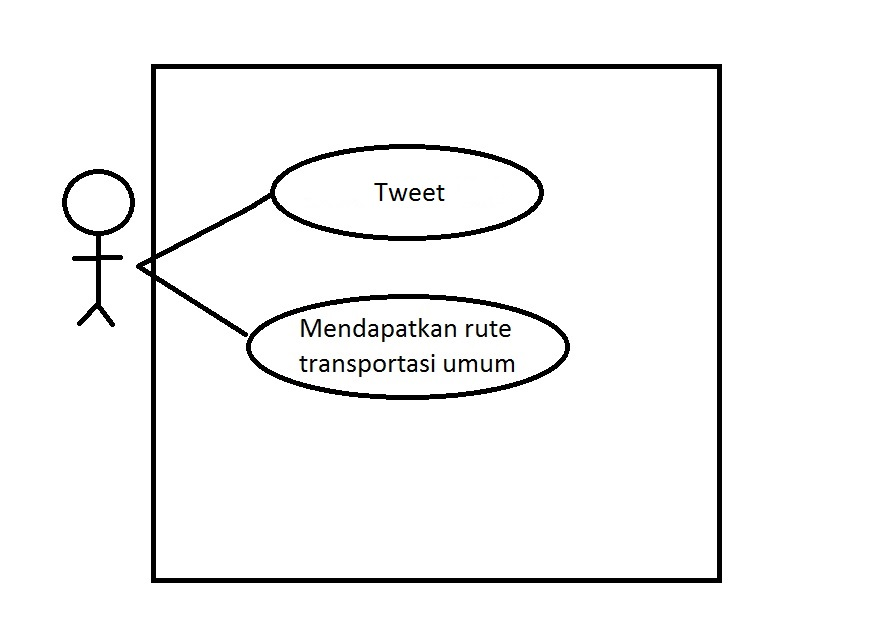
\includegraphics{C:/Users/Kvin/git/Skripsi/doc/DokumenSkripsi/Gambar/usecase.jpg}
	\caption{Use case Twitter Bot}
	\label{fig:usecase}
\end{figure}

\subsubsection{Skenario \textit{Use Case}}
Skenario ini hanya memiliki satu aktor yaitu pengguna. Tweet pada skenario ini dapat dilakukan dengan melakukan tweet kepada user @kiriupdate berisikan format yang sesuai untuk pencarian rute transportasi. 

\begin{table}[h]
\begin{tabular}{|l|l|}
\hline
Nama           & Tweet                                                                                                                          \\ \hline
Aktor          & Pengguna                                                                                                                       \\ \hline
Deskripsi      & \begin{tabular}[c]{@{}l@{}}Melakukan Tweet\\ (Tweet berupa lokasi asal dan lokasi tujuan)\end{tabular}                         \\ \hline
Kondisi Awal   & Belum menuliskan Tweet pada kolom update                                                                                       \\ \hline
Kondisi Akhir  & Sudah melakukan Tweet kepada user @kiriupdate                                                                                  \\ \hline
Skenario Utama & \begin{tabular}[c]{@{}l@{}}Pengguna melakukan Tweet kepada user\\ @kiriupdate dengan format yang sudah ditentukan\end{tabular} \\ \hline
Eksepsi        & Format penulisan salah                                                                                                         \\ \hline
\end{tabular}
\end{table}

\begin{table}[h]
\begin{tabular}{|l|l|}
\hline
Nama           & Mendapatkan rute transportasi umum                                                                                                                                  \\ \hline
Aktor          & Pengguna                                                                                                                                                            \\ \hline
Deskripsi      & \begin{tabular}[c]{@{}l@{}}Tweet balasan yang sudah diolah sedemikian rupa\\ yang berisikan rute transportasi umum dari\\ lokasi awal ke lokasi tujuan\end{tabular} \\ \hline
Kondisi Awal   & Format Tweet kepada user @kiriupdate sudah benar                                                                                                                    \\ \hline
Kondisi Akhir  & Mendapatkan Tweet balasan dari @kiriupdate                                                                                                                          \\ \hline
Skenario Utama & \begin{tabular}[c]{@{}l@{}}Pengguna menerima reply dari user @kiriupdate \\ yang berisikan rute transportasi umum dari\\ lokasi awal ke lokasi tujuan\end{tabular}  \\ \hline
Eksepsi        & Format penulisan salah                                                                                                                                              \\ \hline
\end{tabular}
\end{table}